%!TEX root = ../quantum.tex
\subsubsection{\textcolor{red} {Обозначения Дирака для векторов, волновых функций, операторов и матриц} }


\subsubsection{\textcolor{black} {Стационарные состояния. Энергетическое представление. Различные представления операторов. }}
$$i\hbar\pdv{\Psi(x,t)}{t}=\hat H \Psi(x,t), \text{где } \hat H=-\frac{\hbar^2}{2m}\nabla^2+U(x,t) $$--Уравнение Шредингера, $\hat H$-- оператор Гамильтона

Уравнение Шредингера описывает эволюцию квантово-механической системы. Стационарным называется такое состояние квантово-механической системы, которое не зависит от времени.

$\Psi=\phi(x)\vartheta(t)$-- метод разделения переменных

$$ i\hbar \phi(x)\pdv{\vartheta}{t}=\hat H(\phi(x),\vartheta(t)) $$
$$i\hbar \phi(x)\pdv{\vartheta(t)}{t}=\vartheta(t)\hat H \phi(x) $$
$$i\hbar \frac{\vartheta'}{\vartheta}=\frac{\hat H \phi(x)}{\phi(x)}=E $$

$$\hat{H} \phi(x)=E \phi(x) \label{eq:15.1}$$ -Уравнение на собственные функции.

$$-\frac{\hbar^2}{2m}\dv[2]{\phi(x)}{x}+U(x)\phi(x)=E \phi(x) $$
Решения этого уравнения - пары собственных чисел и собственные функции $E_n \rightarrow \phi_n$.

$\phi_n$ Является базисом, по которому можно раскладывать волновые функции

$\phi \rightarrow E_n$--Дискретный случай

$\phi=\phi(E) $ - Непрерывный случай

Так как есть собственные числа базисной функции $\phi_n$, то разложение по базису $\phi_n$ называется энергетическим представлением.

Найдем энергетическое представление $\Psi_n$
\begin{figure}
\begin{minipage}{0.5\linewidth}
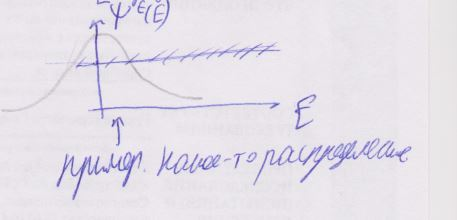
\includegraphics[width=\linewidth]{fig/fig152}
\caption{}
\vspace{-17pt}
\end{minipage}

\begin{minipage}{0.5\linewidth}
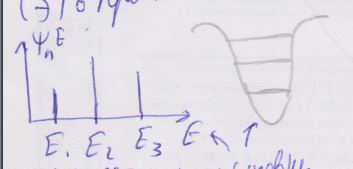
\includegraphics[width=\linewidth]{fig/fig151}
\caption{}
\vspace{-17pt}
\end{minipage}
\end{figure}

\textbf{Дискретный случай}

$$\Psi(x)=\sum\limits_n \phi_n^E \text{--Разложение $\Psi(x)$ по базису $\phi(n)$} $$
$\Psi_n^E$- Волновая функция в E-представлении.


\textbf{Непрерывный случай }
$$\Psi(x)=\infint \Psi^E(E)\phi(x,E)\dd{E} $$

$\Psi_n^E$- Волновая функция в E-представлении.

\subsubsection{\textcolor{black} {Докажите, что собственные значения эрмитового оператора действительны.} }
Рассмотрим уравнение на собственные значения эрмитового оператора $A$
$$
A\ket{\psi_n}=a_n\ket{\psi_n}
$$

Домножим слева скалярно:
$$
\cdot\bra{\psi_m}\bigg|\quad A\ket{\psi_n}=a_n\ket{\psi_n}
$$

Сопряжем эрмитово, сменим индекс и домножим справа:
$$
	\bra{\psi_m}A^+=a_m^+\bra{\psi_m} \quad\bigg|\cdot\ket{\psi_n}
$$

Получим
$$\begin{cases}
	\bra{\psi_m}A\ket{\psi_n}=a_n\bra{\psi_m}\ket{\psi_n}\\
	\bra{\psi_m}A^+\ket{\psi_n}=a_m^+\bra{\psi_m}\ket{\psi_n}
\end{cases}$$

Вычтем одно из другого:
$$
	\bra{\psi_m}A\ket{\psi_n}-\bra{\psi_m}A^+\ket{\psi_n}=
	(a_n-a_m^*)\bra{\psi_m}\ket{\psi_n}
$$

Так как оператор $A$ эрмитов, то $A=A^+\Rightarrow(a_n-a_m^*)\bra{\psi_m}\ket{\psi_n}=0$

Когда $m=n$, $\bra{\psi_m}\ket{\psi_n}\ne0$, и 
$$
	(a_n-a_n^*)=0 \quad\Rightarrow\quad a_n=a_n^*
$$

$\Rightarrow$ собственные значения эрмитова оператора действительны. \qed

